\documentclass{article}
\usepackage{graphicx} % Required for inserting images
\usepackage[T1]{fontenc}
\usepackage{algorithm}
\usepackage{algpseudocode}
\usepackage{multicol}
\usepackage{float}

\title{Obliczenia Naukowe Lista 1}
\author{Maksymilian Neumann}
\date{October 2023}

\begin{document}

\maketitle


\section{Rozpoznanie Arytmetyki}
    Zapoznanie się ze stałymi, limitami i standardem liczb zmienno przecinkowych o standardzie IEEE 754.
\subsection{MACHEPS}
\subsubsection{Opis Problemu}
    Wyznaczenie epsilonu maszynowego dla liczb zmienno przecinkowych. Gdzie $macheps$ to najmniesza liczba taka że, $macheps > 0$ $fl(1.0 + macheps) > 1.0$  i $fl(1.0 + macheps) = 1 + macheps$ tzn. $macheps$ to odległość od 1.0 do kolejnej liczby.
\subsubsection{Rozwiązanie}
    Rozwiązanie zostało napisane w języku Julia i oddane razem ze sprawozdaniem. W którym wyznaczam epsilon maszynowy w sposób iteracyjny.\\ Według następującego schematu:
    \begin{algorithm}
    \caption{Iteracyjny $macheps$}\label{alg:cap}
    \begin{algorithmic}
        \State $x \gets 1.0$
        \State $macheps \gets 1.0$
        \While{ $x + macheps > x$ }
            \State $macheps \gets \frac{macheps}{2}$
        \EndWhile
        \State \textbf{return} $macheps * 2$
    \end{algorithmic}
    \end{algorithm}
\subsubsection{Wyniki i Interpretacja}
    Oto wyniki dla typów Float16, Float32 i Float64
    \begin{center}
        \begin{tabular}{|c||c|c|c|}
        \hline
            Źródło & Float16 & Float32 & Float64 \\
            \hline\hline
            Mój algorytm & 0.000977 & 1.1920929e-7 & 2.220446049250313e-16\\
             \hline
             Funkcja eps() & 0.000977 & 1.1920929e-7 & 2.220446049250313e-16\\
             \hline
             float.h & - & 1.19209e-07 & 2.22045e-16 \\
        \hline
        \end{tabular}
    \end{center}

\subsection{ETA}
\subsubsection{Opis Problemu}
    Wyznaczenie liczby maszynowej $eta$. $eta$ to najmniejsza taka liczba że, $eta > 0.0$
\subsubsection{Rozwiązanie}
    Rozwiązanie zostało napisane w języku Julia i oddane razem ze sprawozdaniem. W którym wyznaczam eta w sposób iteracyjny. Według następującego schematu.
    \begin{algorithm}
    \caption{Iteracyjny $eta$}\label{alg:cap}
    \begin{algorithmic}
        \State $eta \gets 1.0$
        \While{$\frac{eta}{2} > x$} 
            \State $eta \gets \frac{eta}{2}$
        \EndWhile
        \State \textbf{return} $eta$
    \end{algorithmic}
    \end{algorithm}
\subsubsection{Wyniki}
    Oto wyniki dla typów Float16, Float32 i Float64
    \begin{center}
        \begin{tabular}{|c||c|c|c|}
        \hline
            Źródło & Float16 & Float32 & Float64 \\
            \hline\hline
            Mój algorytm & 6.0e-8 & 1.0e-45 & 5.0e-324\\
             \hline
             nextfloat(0.0) & 6.0e-8 & 1.0e-45 & 5.0e-324\\
        \hline
        \end{tabular}
    \end{center}
\subsubsection{Wnioski}
    Liczbę $MIN_{sub}$ oblicza się następująco $MIN_{sub} = 2^{1-t}*2^{c_{min}}$ gdzie $t$ to liczba cyfr mantysy a $c_{min}=-2^{d-1}+2$ gdzie, $d$ oznacza liczbę bitów przeznaczonych na zapis cechy.
        \begin{center}
        \begin{tabular}{|c|c|c|c|}
        \hline
             & Float16 & Float32 & Float64 \\
            \hline
            $MIN_{sub}$ & 6.0e-8 & 1.0e-45 & 5.0e-324\\
        \hline
        \end{tabular}
    \end{center}
    To oznacza ze $eta = MIN_{sub}$
\subsection{MAX}
\subsubsection{Opis Problemu}
    Wyznaczenie liczby $MAX$ tj. maksymalna libcza mnieja niż $\inf$
\subsubsection{Rozwiązanie}
    Rozwiązanie zostało napisane w języku Julia i oddane razem ze sprawozdaniem. W którym wyznaczam eta w sposób iteracyjny. Według następującego schematu.
    \begin{algorithm}
    \caption{Iteracyjny $MAX$}\label{alg:cap}
    \begin{algorithmic}
        \State $MAX \gets prevfloat(1.0)$
        \While{ $MAX * 2 \neq \infty $} 
            \State $MAX \gets MAX * 2$
        \EndWhile
        \State \textbf{return} $MAX$
    \end{algorithmic}
    \end{algorithm}
\subsubsection{Wyniki}
    Oto wyniki dla typów Float16, Float32 i Float64
    \begin{center}
        \begin{tabular}{|c||c|c|c|}
        \hline
            Źródło & Float16 & Float32 & Float64 \\
            \hline\hline
            Mój algorytm & 6.55e4 & 3.4028235e38 & 1.7976931348623157e308\\
             \hline
             floatmax() & 6.55e4 & 3.4028235e38 & 1.7976931348623157e308\\
             \hline
             float.h & - & 3.40282e+38 & 1.79769e+308 \\
        \hline
        \end{tabular}
    \end{center}
\subsection{Wnioski}
        Liczbę $MIN_{nor}$ oblicza się następująco $MIN_{nor} = 2^{c_{min}}$ gdzie $c_{min}$ jest tym samym co przy $MIN_{sub}$ 
        \begin{center}
        \begin{tabular}{|c|c|c|c|}
        \hline
             & Float16 & Float32 & Float64 \\
            \hline
            $MIN_{nor}$ & 6.104e-5 & 1.1754944e-38 & 2.2250738585072014e-308\\
            \hline
            $floatmin()$ & 6.104e-5 & 1.1754944e-38 & 2.2250738585072014e-308\\
        \hline
        \end{tabular}
    \end{center}
    To oznacza ze $eta = MIN_{sub}$
    Po przeprowadzeniu eksperymentów stwierdziłem następujące wnioski:
    \begin{itemize}
        \item Im większa precyzja tym mniejszy $macheps$ 
        \item $MIN_{sub}$ jest równy liczbie eta w danej arytmetyce
        \item $floatmin()$ dla danej arytmetyki jest równy z jej $MIN_{nor}$
    \end{itemize}

\section{Twierdzenie Khan'a}
\subsection{Opis Problemu}
    Nasz problem polega na sprawdzeniu czy Teza Khan'a jest zgodna z rzeczywistością. Brzmi ona tak że można uzyskać epsilon maszynowy obliczając wyrażenie $3.0*(\frac{4.0}{3.0} - 1.0) - 1.0$
\subsection{Rozwiązanie}
    Rozwiązanie zostało napisane w języku Julia i oddane razem ze sprawozdaniem.
\subsection{Wyniki}
    Oto wyniki dla typów Float16, Float32 i Float64
    \begin{center}
        \begin{tabular}{|c||c|c|c|}
        \hline
            Źródło & Float16 & Float32 & Float64 \\
            \hline\hline
            Khan & -0.000977 & 1.1920929e-7 & -2.220446049250313e-16\\
             \hline
             eps() & 0.000977 & 1.1920929e-7 & 2.220446049250313e-16\\
        \hline
        \end{tabular}
    \end{center}
\subsection{Wnioski}
    Wyniki z wyrażenia od Khan'a są identyczne jeśli chodzi o wartość bezwzględną różnią się znakiem dla Float16 i Float64
    
\section{Rozmieszczenie Floatów w Przedziale}
\subsection{Opis Problemu}
Rozważamy rozmieszczenie liczb zmiennoprzecinkowych Float64 w standardzie IEEE 754 w przedziale [1, 2]. Czy liczbyw w tym przedziale są równomiernie rozmieszczone z krokiem $\delta=2^{-52}$
\subsection{Rozwiązanie}
    Rozwiązanie polega na tym że zwiększamy naszą początkową liczbę o $\delta$ i obserwujemy jej reprezentacje binarną oraz porównujemy wyniki z wynikami reprezentacji po funkcji $nextfloat()$.
\subsection{Wyniki}
Wyniki gdzie $\delta=2^{-52}$: 
Następne 4 liczb po 1:\\
0011111111110000000000000000000000000000000000000000000000000000\\
0011111111110000000000000000000000000000000000000000000000000001\\
0011111111110000000000000000000000000000000000000000000000000010\\
0011111111110000000000000000000000000000000000000000000000000011\\
0011111111110000000000000000000000000000000000000000000000000100\\
Następne 4 delta większych po 1:\\
0011111111110000000000000000000000000000000000000000000000000000\\
0011111111110000000000000000000000000000000000000000000000000001\\
0011111111110000000000000000000000000000000000000000000000000010\\
0011111111110000000000000000000000000000000000000000000000000011\\
0011111111110000000000000000000000000000000000000000000000000100\\
Następne 4 liczb po 0.5:\\
0011111111100000000000000000000000000000000000000000000000000000\\
0011111111100000000000000000000000000000000000000000000000000001\\
0011111111100000000000000000000000000000000000000000000000000010\\
0011111111100000000000000000000000000000000000000000000000000011\\
0011111111100000000000000000000000000000000000000000000000000100\\
Następne 4 delta większych po 0.5:\\
0011111111100000000000000000000000000000000000000000000000000000\\
0011111111100000000000000000000000000000000000000000000000000010\\
0011111111100000000000000000000000000000000000000000000000000100\\
0011111111100000000000000000000000000000000000000000000000000110\\
0011111111100000000000000000000000000000000000000000000000001000\\
Następne 4 liczb po 2:\\
0100000000000000000000000000000000000000000000000000000000000000\\
0100000000000000000000000000000000000000000000000000000000000001\\
0100000000000000000000000000000000000000000000000000000000000010\\
0100000000000000000000000000000000000000000000000000000000000011\\
0100000000000000000000000000000000000000000000000000000000000100\\
Następne 4 delta większych po 0.5:\\
0100000000000000000000000000000000000000000000000000000000000000\\
0100000000000000000000000000000000000000000000000000000000000000\\
0100000000000000000000000000000000000000000000000000000000000000\\
0100000000000000000000000000000000000000000000000000000000000000\\
0100000000000000000000000000000000000000000000000000000000000000\\
\subsection{Wnioski}
Dla przedziału [1, 2] rozmieszczenie liczb jest równomiernie z $\delta=2^{-52}$ dla przedziału [.5, 1] $\delta$ jest mniejsz a dla [2, 4] jest większa.
\section{Niezgodność Wyniku z Teorią}
\subsection{Opis Problemu}
    Znalezienie liczby w arytmetyce Float64 liczbe $x$ w przedziale $1<x<2$ taką, że $x*(1/x) \neq 1$.
\subsection{Rozwiązanie}
    Rozwiązanie zostało napisane w języku Julia. Według następującej procedury.
    \begin{algorithm}
    \caption{Zad. 4}\label{alg:cap}
    \begin{algorithmic}
        \State $x \gets nextfloat(1.0)$
        \While{ $x < 2$} 
            \If{$(x * ( 1 / x)) \neq 1 $}
                \State \textbf{return} $x$
            \EndIf
            \State $x \gets nextfloat(x)$
        \EndWhile
    \end{algorithmic}
    \end{algorithm}
\subsection{Wyniki}
Pierwsze 10 wartości:
\begin{multicols}{2}
\begin{enumerate}
    \item 1.000000057228997
    \item 1.000000066222211
    \item 1.0000000694943918
    \item 1.0000000710740116
    \item 1.0000000833000269
    \item 1.0000000991235327
    \item 1.000000105103379
    \item 1.0000001071951936
    \item 1.00000011025853
    \item 1.0000001151831874
\end{enumerate}
\end{multicols}
\subsection{Wnioski}
    Najmniejsza taka liczba to 1.000000057228997. Istnienie takich liczb wynika z reprezentacji ich w standardzie IEEE 754 i zaokrąglaniu podczas działań.

\section{Iloczyn Skalarny Dwuch Wektorów}
\subsection{Opis Problemu}
    Znalezienie różnic między implementacjami Iloczynów Skalarnych dwuch wektorów na przykładzie:\\ x = [2.718281828, -3.141592654, 1.414213562, 0.5772156649, 0.3010299957]\\
    y = [1486.2497, 878366.9879, -22.37492, 4773714.647, 0.000185049]
\subsection{Rozwiązanie}
    Rozwiązanie wykonane w języku Julia. Według następujących rozumowań:
    \begin{enumerate}
        \item "w przód" t.j. $\sum^n_{i=1} x_i y_i$
        \item "w tył" t.j. $\sum^1_{i=n} x_i y_i$
        \item "od największego do najmniejszego"
        \item "od najmniejszego do największego"
    \end{enumerate}
\subsection{Wyniki}
    Uzyskałem następujące wyniki. I porównałem z prawidłową wartością.
    \begin{center}
        \begin{tabular}{|c||c|c|c|}
        \hline
            Źródło & Float32 & Float64 & Rzeczywista \\
            \hline\hline
            "1" & -0.3472038161853561 & 1.0251881368296672e-10 & -1.00657107000000e-11\\
             \hline
             "2" & 0.0 & 0.0 & -1.00657107000000e-11\\
             \hline
             "3"& -0.3472038162872195 & 0.0 & -1.00657107000000e-11\\
             \hline
             "4"& -0.3472038162872195 & 0.0 & -1.00657107000000e-11\\
        \hline
        \end{tabular}
    \end{center}
\subsection{Wnioski}

\section{Ta Sama Funkcja Inny Wynik}
\subsection{Opis Problemu}
    Porównanie wyników funkcji $f(x) = g(x)$ gdzie:\\
    \begin{center}
        $f(x)=\sqrt{x^2 + 1} - 1$\\ $g(x)=\frac{x^2}{\sqrt{x^2 +1}+1}$
    \end{center}
\subsection{Rozwiązanie}
    Dla $x$ = $8^{-1}$, $8^{-2}$, $8^{-3}$, ... liczymy f(x) i g(x) wyniki porównujemy. Wszystko jest liczone na Float64 w języku Julia.
\subsection{Wyniki}
        \begin{center}
        \begin{tabular}{|c||c|c|}
        \hline
            $x$ & $f(x)$ & $g(x)$ \\
            \hline\hline
            $8^{-1}$ & -0.875 & 0.0077822185373187065 \\
             \hline
             $8^{-2}$ & -0.984375 & 0.00012206286282875901\\
             \hline
             $8^{-3}$ & -0.998046875 & 1.907346813826566e-6\\
             \hline
             $8^{-4}$ & -0.999755859375 & 2.9802321943606116e-8\\
            \hline
             $8^{-5}$ & -0.999969482421875 & 4.6566128719931904e-10\\
        \hline
        \end{tabular}
    \end{center}
\subsection{Wnioski}
    Wiarygodnymi wynikami są wyniki funkcji $g(x)$ ponieważ funkcja $f(x)$ zwraca nam wyniki ujemne gdzie w rzeczywistości są one nieujemne.

\section{Estymacja Pochodnej w Punkcie}
\subsection{Opis Problemu}
    Przybliżoną wartość pochodnej $f(x)$ w punkcie $x$ można obliczyć za pomocą następującego wzoru:\\
    \begin{center}
        $f^{'}(x_0)\approx\tilde{f^{'}}(x_0) = \frac{f(x_0+h) - f(x_0)}{h}$
    \end{center}
    Kożystając z niego aproksymujemy $f(x)=sinx+cos3x$ w punkcie $x_0 = 1$ oraz obliczamy błedy $|f^{'}(x_0) - \tilde{f^{'}}(x_0)|$ dla $h=2^{-n}$ (n = 0, 1, 2, ..., 54)
\subsection{Rozwiązanie}
    Rozwiązanie zostało napisane w Języku Julia dla typu Float64 polegające na porównywaniu wyników dokładnych z przybliżonymi według wzoru podanego wyżej i odesłane razem ze sprawozdaniem.
\subsection{Wyniki}
Jak można zauważyć w poniższej figurze wielkość błędu przy zmniejszającym się $h$ zmiejsza się tylko do pewnego momętu a następnie zaczyna wzrastać.
    \begin{figure}[H]
        \centering
        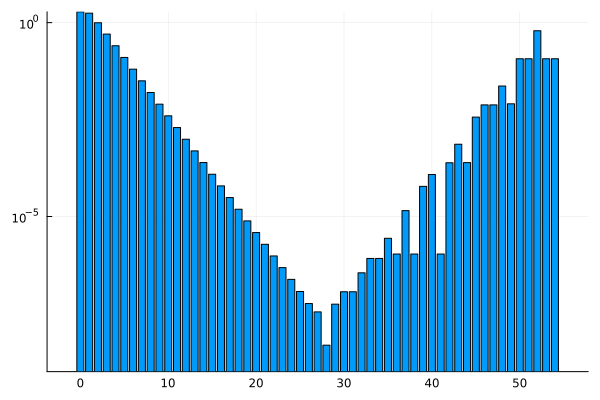
\includegraphics[width=0.75\linewidth]{7.png}
        \caption{Wielkość Błędu}
        \label{fig:enter-label}
    \end{figure}
\subsection{Wnioski}
    Uzyskane dane i dysonans związany z tym że intuicyjnie przy zmiejszającym się $h$ zmiejszać powinien się błąd wynika z tego że $1+h$ zmierza do $1$ przy czym $f(1+h) - f(1)$ zmierza do $0$ i dzielimy to przez $h$ któte również zmierza do $0$ narażając się na błedy związane z artymetyką zmiennoprzecinkową.
\end{document}
